\documentclass{beamer}\usepackage[]{graphicx}\usepackage[]{color}
% maxwidth is the original width if it is less than linewidth
% otherwise use linewidth (to make sure the graphics do not exceed the margin)
\makeatletter
\def\maxwidth{ %
  \ifdim\Gin@nat@width>\linewidth
    \linewidth
  \else
    \Gin@nat@width
  \fi
}
\makeatother

\definecolor{fgcolor}{rgb}{0.345, 0.345, 0.345}
\newcommand{\hlnum}[1]{\textcolor[rgb]{0.686,0.059,0.569}{#1}}%
\newcommand{\hlstr}[1]{\textcolor[rgb]{0.192,0.494,0.8}{#1}}%
\newcommand{\hlcom}[1]{\textcolor[rgb]{0.678,0.584,0.686}{\textit{#1}}}%
\newcommand{\hlopt}[1]{\textcolor[rgb]{0,0,0}{#1}}%
\newcommand{\hlstd}[1]{\textcolor[rgb]{0.345,0.345,0.345}{#1}}%
\newcommand{\hlkwa}[1]{\textcolor[rgb]{0.161,0.373,0.58}{\textbf{#1}}}%
\newcommand{\hlkwb}[1]{\textcolor[rgb]{0.69,0.353,0.396}{#1}}%
\newcommand{\hlkwc}[1]{\textcolor[rgb]{0.333,0.667,0.333}{#1}}%
\newcommand{\hlkwd}[1]{\textcolor[rgb]{0.737,0.353,0.396}{\textbf{#1}}}%
\let\hlipl\hlkwb

\usepackage{framed}
\makeatletter
\newenvironment{kframe}{%
 \def\at@end@of@kframe{}%
 \ifinner\ifhmode%
  \def\at@end@of@kframe{\end{minipage}}%
  \begin{minipage}{\columnwidth}%
 \fi\fi%
 \def\FrameCommand##1{\hskip\@totalleftmargin \hskip-\fboxsep
 \colorbox{shadecolor}{##1}\hskip-\fboxsep
     % There is no \\@totalrightmargin, so:
     \hskip-\linewidth \hskip-\@totalleftmargin \hskip\columnwidth}%
 \MakeFramed {\advance\hsize-\width
   \@totalleftmargin\z@ \linewidth\hsize
   \@setminipage}}%
 {\par\unskip\endMakeFramed%
 \at@end@of@kframe}
\makeatother

\definecolor{shadecolor}{rgb}{.97, .97, .97}
\definecolor{messagecolor}{rgb}{0, 0, 0}
\definecolor{warningcolor}{rgb}{1, 0, 1}
\definecolor{errorcolor}{rgb}{1, 0, 0}
\newenvironment{knitrout}{}{} % an empty environment to be redefined in TeX

\usepackage{alltt}
\usepackage{../371g-slides}
\title{Bayes' Rule \& Random Variables}
\subtitle{Lecture 4}
\author{STA 371G}
\IfFileExists{upquote.sty}{\usepackage{upquote}}{}
\begin{document}




\frame{\maketitle}

\AtBeginSection[]{
    \begin{frame}<beamer>
      \tableofcontents[currentsection]
    \end{frame}
  }

\begin{darkframes}

\begin{frame}{Announcements}
  \begin{itemize}
    \item Homework 1 is due tonight at 11:59 PM (through MyStatLab)
    \item Quiz 1 is Tuesday night at 6:30 PM (covers material through last week --- not today)
  \end{itemize}
\end{frame}

\section{Bayes' Rule}

\begin{frame}{COVID testing}
  \begin{itemize}[<+->]
    \item COVID testing is important for public health, but COVID tests are not perfect
    \item The Beckman Coulter Access SARS-CoV-2 IgG test has the following properties:
      \begin{itemize}
        \item If you \textbf{have COVID}, there is a 96.8\% chance the test will show a \textbf{positive result}
        \item If you \textbf{do not have COVID}, there is a 99.6\% chance the test will show a \textbf{negative result}
      \end{itemize}
    \item Let's suppose that 1\% of people in the population being tested actually have COVID
  \end{itemize}
\end{frame}

\begin{frame}{COVID testing}
  \begin{center}
    \[
      C = \text{has COVID}, \qquad T = \text{tests positive for COVID}
    \]
    We know $P(T|C) = 0.968$, but we really want to know is $P(C|T)$!
  \end{center}
\end{frame}

\begin{frame}{Bayes Rule}
  For any events $A$ and $B$,
  \begin{eqnarray*}
    P(A|B) &=& \dfrac{P(\text{$A$ and $B$})}{P(B)} \\ \pause 
    &=& \dfrac{P(B|A)P(A)}{P(\text{$B$ and $A$}) + P(\text{$B$ and $A^c$})} \\ \pause
    &=& \dfrac{P(B|A)P(A)}{P(B|A)P(A) + P(B|A^c)P(A^c)}
  \end{eqnarray*}
  \pause
  Bayes Rule allows us to ``reverse the conditioning'' and find $P(A|B)$ when we know $P(B|A)$.
\end{frame}

\begin{frame}{COVID testing}
  Bayes Rule says
  \[
    P(C|T) = \frac{P(T|C)P(C)}{P(T|C)P(C) + P(T|C^c)P(C^c)}
  \]

  We know
  \[ P(T|C) = 0.968, \qquad P(T^c|C^c) = 0.996, \qquad P(C) = 0.01 \]

  \pause

  So:
  \begin{itemize}[<+->]
    \item $P(C^c) = 1-P(C) = 0.99$
    \item $P(T|C^c) = 1-P(T^c|C^c) = 0.004$
  \end{itemize}
\end{frame}

\begin{frame}{COVID testing}


\begin{align*}
  P(C|T) &= \frac{ P(T|C)P(C) }{ P(T|C)P(C) + P(T|C^c)P(C^c) } \\
  &= \frac{ (0.968)(0.01) }{ (0.968)(0.01) + (0.004)(0.99) } \\
  &= 0.71
\end{align*}
\end{frame}

\begin{frame}{COVID testing}
  \begin{itemize}[<+->]
    \item If you have COVID, there is a 96.8\% chance the test will show a positive result
    \item If you do not have HIV, there is a 99.6\% chance the test will show a negative result
    \item But if you test positive there is only a 71\% chance you have COVID!
    \item This is counterintuitive, and is due to the low 1\% ``base rate'' of people that actually COVID
    \item It's surprisingly low because of the way we as humans are wired (it even has a name: ``base rate fallacy'')
  \end{itemize}
\end{frame}

\begin{frame}{Another way to look at it}
  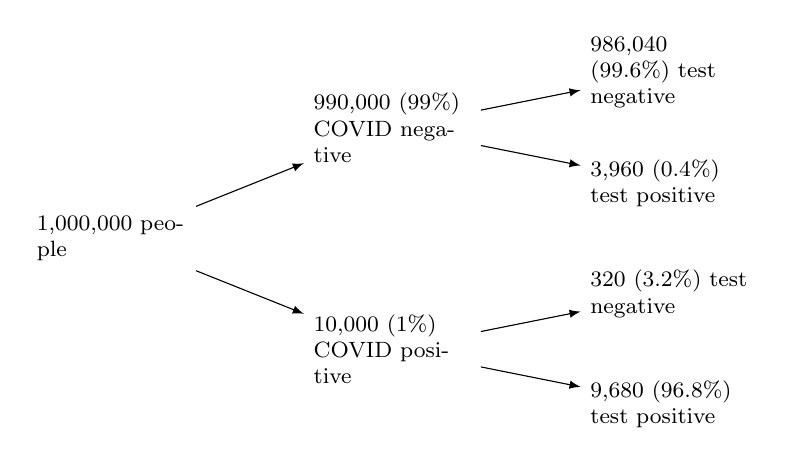
\begin{tikzpicture}
  [
    grow                    = right,
    sibling distance        = 8em,
    level distance          = 10em,
    level 2/.style          = { sibling distance=4em },
    edge from parent/.style = {draw, -latex},
    every node/.style       = {font=\footnotesize, text width=2 cm},
    sloped
  ]
  \node { 1,000,000 people }
  child {
    node { 10,000 (1\%) COVID positive }
    child {
      node { 9,680 (96.8\%) test positive }
    }
    child {
      node { 320 (3.2\%) test negative }
    }
  }
  child {
    node { 990,000 (99\%) COVID negative }
    child {
      node { 3,960 (0.4\%) test positive }
    }
    child {
      node { 986,040 (99.6\%) test negative }
    }
  };
  \end{tikzpicture}
  \pause

  Of the $9680+3960=13640$ people that tested positive, only $9680$ (71\%) are actually COVID positive!
  
\end{frame}

\begin{frame}
  Think of Bayes' Rule as a way to update our thinking based on new information:

  \bigskip

  \begin{center}
    \begin{tabular}{ll}
      $P(C)$ & $\longleftarrow$ Prior probability \\
      $P(C|T)$ & $\longleftarrow$ Posterior probability (includes new information) \\
    \end{tabular}
  \end{center}
  
\end{frame}

\begin{frame}
  \fullpagepicture{doctors}
\end{frame}

\begin{frame}
  Just 21\% of gynecologists got the right answer!
  \bigskip\pause

  In other words, this is hard, and it goes against our intuition!
\end{frame}

\section{Discrete random variables}

\begin{frame}{Random variables}
  \begin{definition}
    A \alert{random variable} is a variable that can take on different numeric values with different probabilities. 
    The \alert{distribution} of a random variable indicates each possible outcome with its corresponding probability.
  \end{definition}
\end{frame}

\begin{frame}{iPhone prices}
  Let $T$ be the possible prices, in dollars, of a randomly-selected iPhone 12 sold in October-November 2020.
  The probabilities come from the actual percentage sold: 

  \begin{center}
    \begin{tabular}{lll}
      Model & Price ($x$) & $P(T=x)$ \\
      \hline
      iPhone 12 & \$799 & 0.35 \\
      iPhone 12 Pro & \$999 & 0.29 \\
      iPhone 12 Pro Max & \$1,099 & 0.28 \\
      iPhone 12 Mini & \$699 & 0.08 \\
    \end{tabular}
  \end{center}

  \pause
  How would we quantify the price of a ``typical'' or ``average'' iPhone 12? And how would we quantify how different the prices paid by different customers are?
\end{frame}

\begin{frame}{Expected value}
  The expected value represents the long-run average price if we selected iPhones over and over an infinite number of times:
  \begin{align*}
    E(T) &= \sum_{\text{All prices $x$}} x \cdot P(T = x) \\
    &= 700 \cdot 0.35 + 999 \cdot 0.29 + 1099 \cdot 0.28 + 699 \cdot 0.08 \\
    &= \$933.
  \end{align*}
  It can be thought of as the price of a ``typical'' iPhone.
\end{frame}

\begin{frame}[fragile]{Calculating expected values in R}
  In R, define the probabilities and values (prices) in separate vectors:
\begin{knitrout}
\definecolor{shadecolor}{rgb}{0.969, 0.969, 0.969}\color{fgcolor}\begin{kframe}
\begin{alltt}
\hlstd{prices} \hlkwb{<-} \hlkwd{c}\hlstd{(}\hlnum{799}\hlstd{,} \hlnum{999}\hlstd{,} \hlnum{1099}\hlstd{,} \hlnum{699}\hlstd{)}
\hlstd{probs} \hlkwb{<-} \hlkwd{c}\hlstd{(}\hlnum{0.35}\hlstd{,} \hlnum{0.29}\hlstd{,} \hlnum{0.28}\hlstd{,} \hlnum{0.08}\hlstd{)}

\hlcom{# Calculate expected value}
\hlkwd{sum}\hlstd{(prices} \hlopt{*} \hlstd{probs)}
\end{alltt}
\begin{verbatim}
[1] 933
\end{verbatim}
\end{kframe}
\end{knitrout}
\end{frame}

\begin{frame}{Variance and standard deviation}
  The variance and standard deviation represents the long-run variance and standard deviation of the prices of an infinite number of iPhones selected at random:
  \begin{align*}
    \text{Var}(T) &= \sum_{\text{All prices $x$}} (x - E(T))^2 \cdot P(T=x) \\
    &= (700-933)^2\cdot 0.35 + (999-933)^2\cdot 0.29 + \\
    &\qquad (1099-933)^2\cdot 0.28 + (699-933)^2\cdot 0.08 \\
    &= 19644 \\
    \text{SD}(T) &= \sqrt{\text{Var}(T)} \\
    &= \$140.16.
  \end{align*}
\end{frame}

\begin{frame}[fragile]{Calculating variance and SD in R}
\begin{knitrout}
\definecolor{shadecolor}{rgb}{0.969, 0.969, 0.969}\color{fgcolor}\begin{kframe}
\begin{alltt}
\hlcom{# Expected value}
\hlstd{iphone.ev} \hlkwb{<-} \hlkwd{sum}\hlstd{(prices} \hlopt{*} \hlstd{probs)}
\hlcom{# Variance}
\hlstd{iphone.var} \hlkwb{<-} \hlkwd{sum}\hlstd{((prices} \hlopt{-} \hlstd{iphone.ev)}\hlopt{^}\hlnum{2} \hlopt{*} \hlstd{probs)}
\hlstd{iphone.var}
\end{alltt}
\begin{verbatim}
[1] 19644
\end{verbatim}
\begin{alltt}
\hlcom{# Standard deviation}
\hlkwd{sqrt}\hlstd{(iphone.var)}
\end{alltt}
\begin{verbatim}
[1] 140
\end{verbatim}
\end{kframe}
\end{knitrout}
\end{frame}

\section{Continuous random variables: Normal distributions}

\begin{frame}[fragile]{Data set}
  The data set \texttt{ut2000} contains information on all 5191 students that entered UT Austin in Fall 2000 and graduated within 6 years.
\begin{knitrout}
\definecolor{shadecolor}{rgb}{0.969, 0.969, 0.969}\color{fgcolor}\begin{kframe}
\begin{alltt}
\hlkwd{head}\hlstd{(ut2000)}
\end{alltt}
\begin{verbatim}
  SAT.V SAT.Q SAT.C          School GPA Status
1   690   580  1270        BUSINESS 3.8      G
2   530   710  1240 NATURAL SCIENCE 3.5      G
3   610   700  1310 NATURAL SCIENCE 3.4      G
4   730   700  1430     ENGINEERING 3.3      G
5   700   710  1410 NATURAL SCIENCE 3.7      G
6   540   690  1230    LIBERAL ARTS 2.7      G
\end{verbatim}
\end{kframe}
\end{knitrout}
  \footnotesize{Data from James Scott: \url{http://jgscott.github.io/teaching/data/ut2000.csv}}
\end{frame}
  
\begin{frame}{In the year 2000...}
  \begin{itemize}[<+->]
    \item The most popular TV show was \emph{Survivor}
    \item Britney Spears' \emph{Oops!...I did it again} had just come out
    \item Angelina Jolie was married to Billy Bob Thorton
    \item I was a college freshman
  \end{itemize}
\end{frame}
  
\begin{frame}[fragile]
\begin{knitrout}
\definecolor{shadecolor}{rgb}{0.969, 0.969, 0.969}\color{fgcolor}\begin{kframe}
\begin{alltt}
\hlkwd{hist}\hlstd{(ut2000}\hlopt{$}\hlstd{SAT.C,} \hlkwc{main}\hlstd{=}\hlstr{""}\hlstd{,} \hlkwc{col}\hlstd{=}\hlstr{"orange"}\hlstd{,} \hlkwc{xlab}\hlstd{=}\hlstr{"SAT"}\hlstd{)}
\end{alltt}
\end{kframe}
\includegraphics[width=\maxwidth]{/tmp/figures/unnamed-chunk-6-1} 

\end{knitrout}
\end{frame}

\begin{frame}[fragile]
  This random variable is approximately \alert{Normal}, with mean $\mu=1215.03$ and SD $\sigma=145.38$:

\begin{knitrout}
\definecolor{shadecolor}{rgb}{0.969, 0.969, 0.969}\color{fgcolor}
\includegraphics[width=\maxwidth]{/tmp/figures/unnamed-chunk-7-1} 

\end{knitrout}
\end{frame}

\begin{frame}{The Empirical Rule}
  \begin{itemize}
    \item About 68\% of a Normal random variable falls within $\pm 1$ SD of the mean
    \item About 95\% of a Normal random variable falls within $\pm 2$ SD of the mean
    \item About 99.7\% of a Normal random variable falls within $\pm 3$ SD of the mean
  \end{itemize}
\end{frame}

\begin{frame}{The Empirical Rule}
  \begin{itemize}[<+->]
    \item About 68\% of students scored between $1215.03 - 145.38 = 1069.65$ and $1215.03 + 145.38  = 1360.41$
    \item About 95\% of students scored between $1215.03 - 2\cdot145.38 = 924.27$ and $1215.03 + 2\cdot145.38  = 1505.79$
    \item About 99.7\% of students scored between $1215.03 - 3\cdot145.38 = 778.89$ and $1215.03 + 3\cdot145.38  = 1651.17$
  \end{itemize}
\end{frame}

\begin{frame}[fragile]{Calculating probabilities using R}
  The \texttt{pnorm($x$, $\mu$, $\sigma$)} function calculates $P(X < x)$ if $X$ is a Normal random variable with mean $\mu$ and SD $\sigma$.
\end{frame}

\begin{frame}
\begin{knitrout}
\definecolor{shadecolor}{rgb}{0.969, 0.969, 0.969}\color{fgcolor}
\includegraphics[width=\maxwidth]{/tmp/figures/unnamed-chunk-8-1} 

\end{knitrout}
  \begin{center}
    $P(\text{SAT}<1000) = $ \texttt{pnorm(1000, 1215.03, 145.38)} $ = 0.07$ 
  \end{center}
\end{frame}

\begin{frame}
\begin{knitrout}
\definecolor{shadecolor}{rgb}{0.969, 0.969, 0.969}\color{fgcolor}
\includegraphics[width=\maxwidth]{/tmp/figures/unnamed-chunk-9-1} 

\end{knitrout}
  \begin{center}
    $P(\text{SAT}>1500) = $ \texttt{1 - pnorm(1500, 1215.03, 145.38)} $ = 0.02$ 
  \end{center}
\end{frame}

\begin{frame}[fragile]
\begin{knitrout}
\definecolor{shadecolor}{rgb}{0.969, 0.969, 0.969}\color{fgcolor}
\includegraphics[width=\maxwidth]{/tmp/figures/unnamed-chunk-10-1} 

\end{knitrout}

  \[
    P(1100<\text{SAT}<1400) = \text{?}
  \]
\end{frame}

\begin{frame}{How to tell if data is Normal?}
  Variables can fail to be Normal in multiple ways:
  \begin{enumerate}
    \item Normal random variables are \alert{unimodal}; multimodal random variables are not Normal
    \item Normal random variables are \alert{symmetric}; skewed random variables are not Normal
    \item Normal random variables have a \alert{bell shape}; random variables with extreme outliers (or tails that are too ``fat'' or too ``skinny'') are not Normal
  \end{enumerate}
\end{frame}

\begin{frame}[fragile]{Checking for normality in R}
  The \texttt{qqnorm} function creates a Normal probability plot; a perfectly Normal distribution will have a straight line.
\begin{knitrout}
\definecolor{shadecolor}{rgb}{0.969, 0.969, 0.969}\color{fgcolor}\begin{kframe}
\begin{alltt}
\hlkwd{qqnorm}\hlstd{(ut2000}\hlopt{$}\hlstd{SAT.C)}
\end{alltt}
\end{kframe}
\includegraphics[width=\maxwidth]{/tmp/figures/unnamed-chunk-11-1} 

\end{knitrout}
\end{frame}

\begin{frame}[fragile]{Checking for normality in R}
  The \alert{skewness} measures skewness; it is negative for left-skewed distributions, symmetric for symmetric distributions, and positive for right-skewed distributions.
\begin{knitrout}
\definecolor{shadecolor}{rgb}{0.969, 0.969, 0.969}\color{fgcolor}\begin{kframe}
\begin{alltt}
\hlkwd{library}\hlstd{(moments)}
\hlkwd{skewness}\hlstd{(ut2000}\hlopt{$}\hlstd{SAT.C)}
\end{alltt}
\begin{verbatim}
[1] -0.1
\end{verbatim}
\end{kframe}
\end{knitrout}
\end{frame}

\begin{frame}[fragile]{Checking for normality in R}
  The \alert{kurtosis} is $<3$ for distributions with skinny tails, $=3$ for Normal distributions, and $>3$ for distributions with fat tails.
\begin{knitrout}
\definecolor{shadecolor}{rgb}{0.969, 0.969, 0.969}\color{fgcolor}\begin{kframe}
\begin{alltt}
\hlkwd{kurtosis}\hlstd{(ut2000}\hlopt{$}\hlstd{SAT.C)}
\end{alltt}
\begin{verbatim}
[1] 2.9
\end{verbatim}
\end{kframe}
\end{knitrout}
\end{frame}

\begin{frame}{Checking for normality in R}
  The Q-Q plot is almost a straight line, the skewness is almost exactly 0, and the kurtosis is almost exactly 3, so the SAT distribution is almost exactly Normal.
\end{frame}

\end{darkframes}
\end{document}
